\begin{frame}{Let's Take a Step Back}
\begin{table}
\centering
\begin{tabular}{cc}
Model Overconfidence & Rubbish Examples \\
\cite{guo2017calibration} & \cite{goodfellow2014explaining} \\
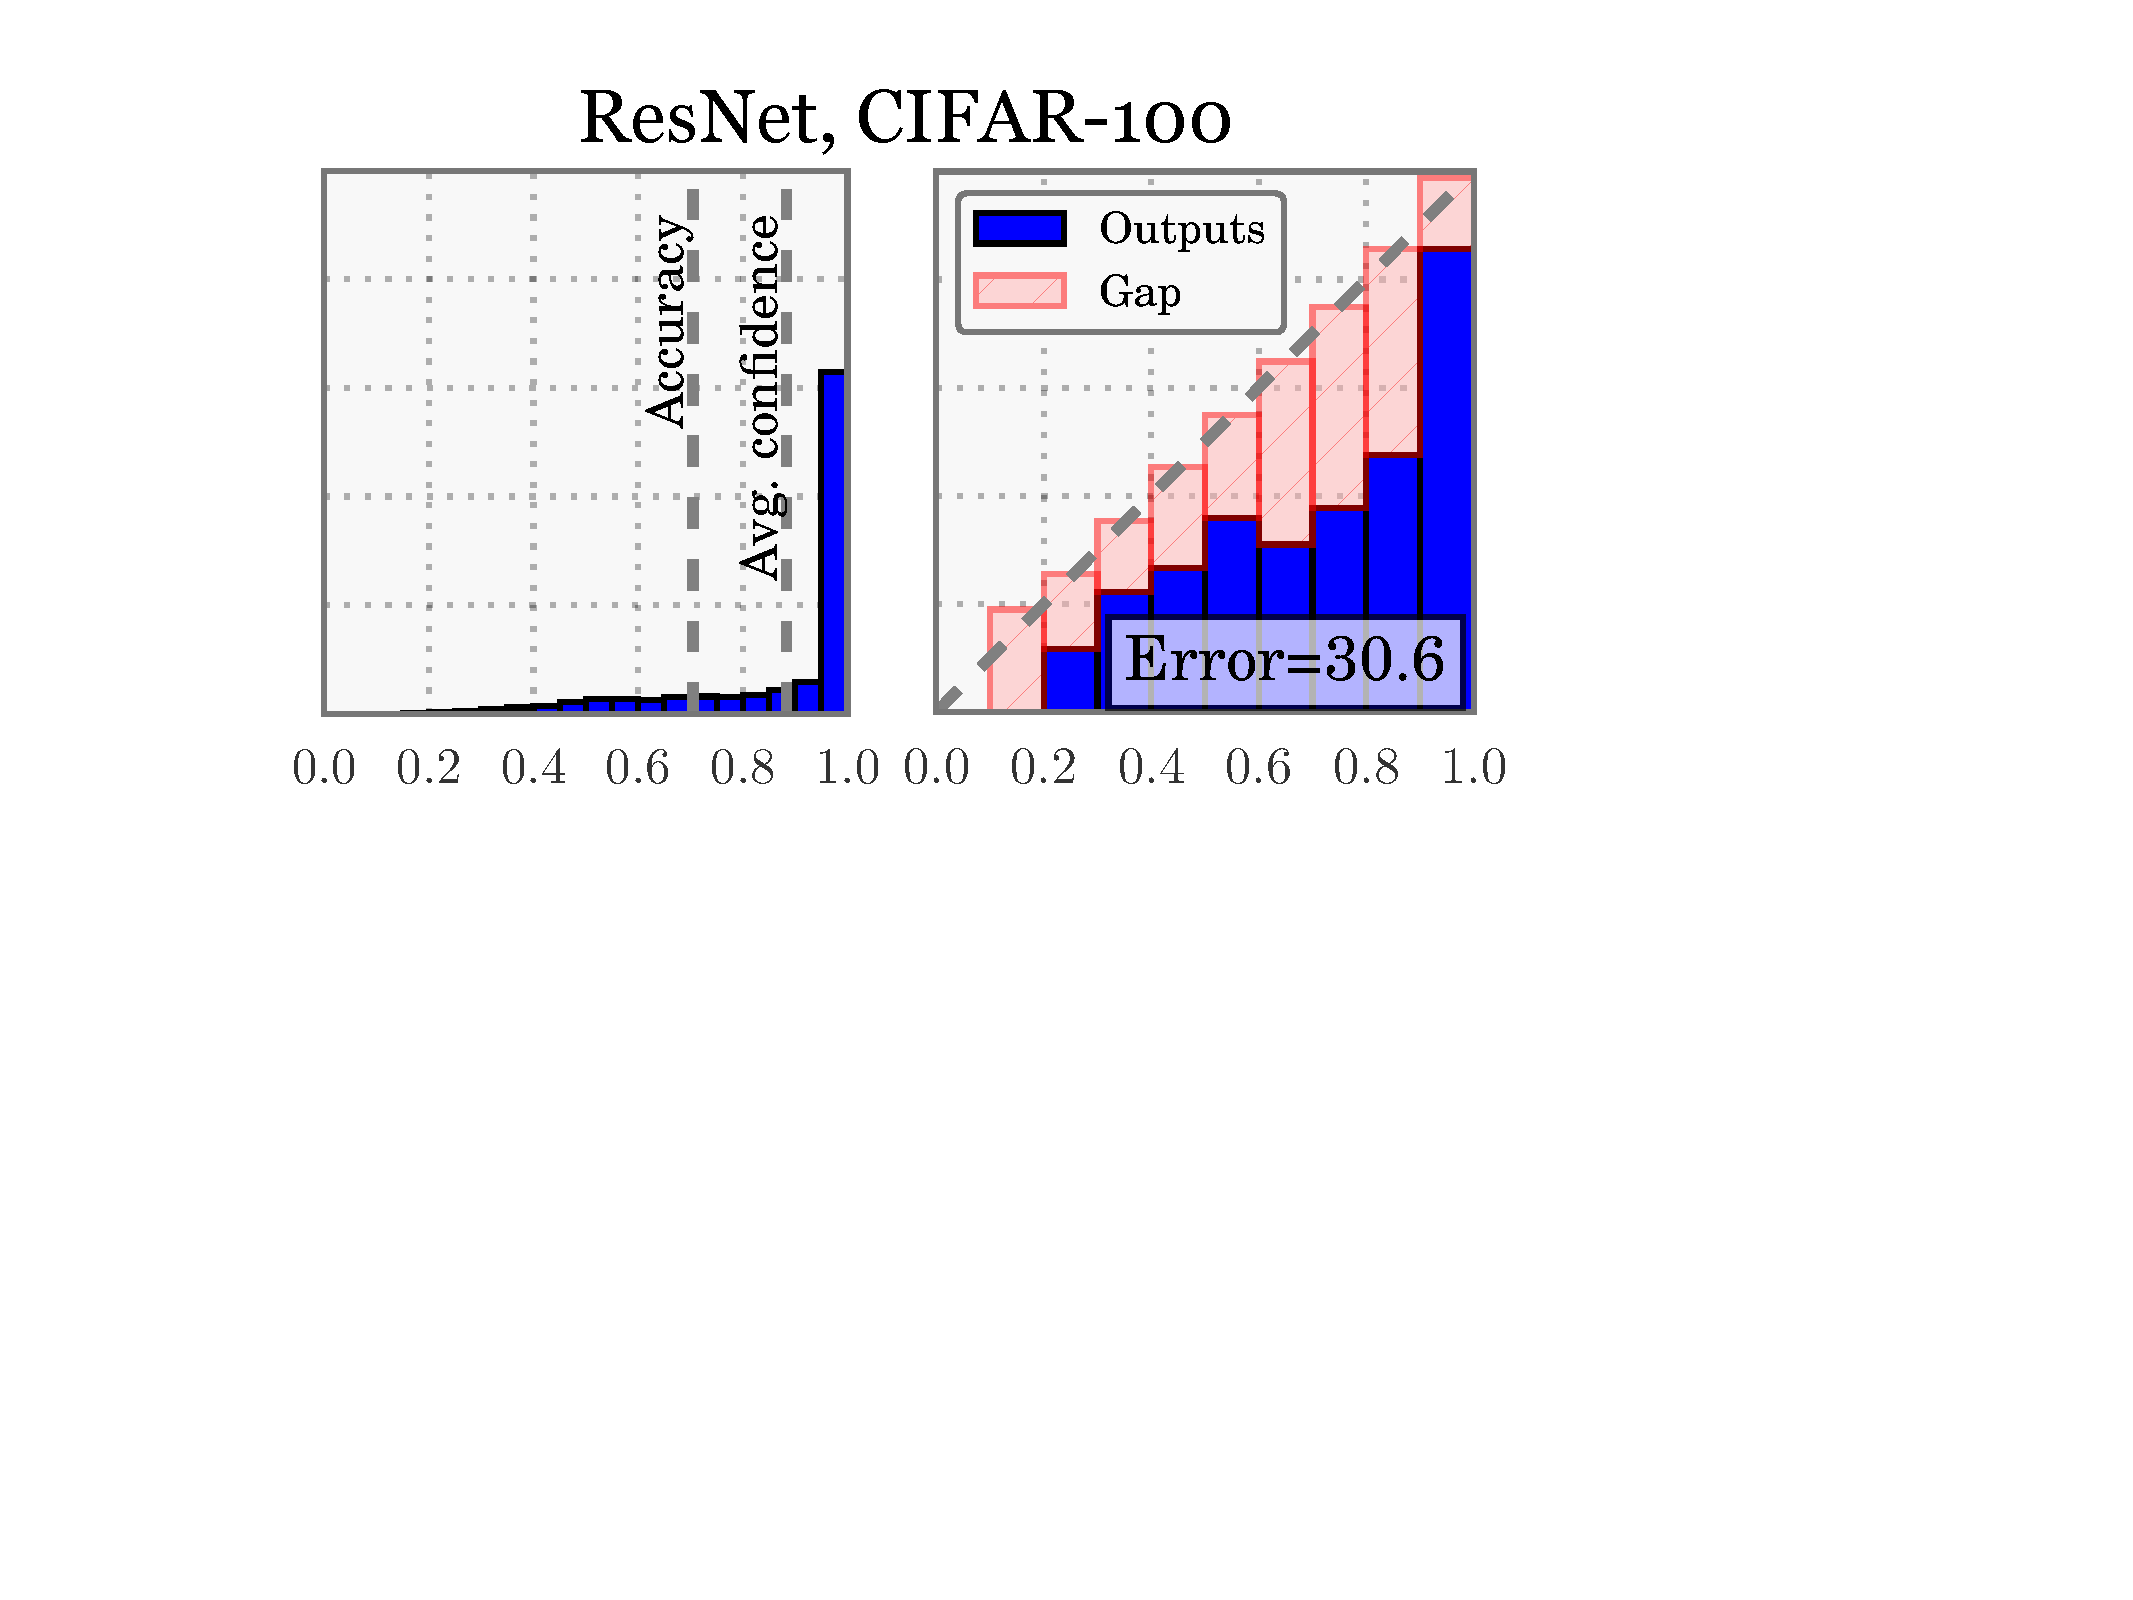
\includegraphics[height=2.5cm]{guo} & 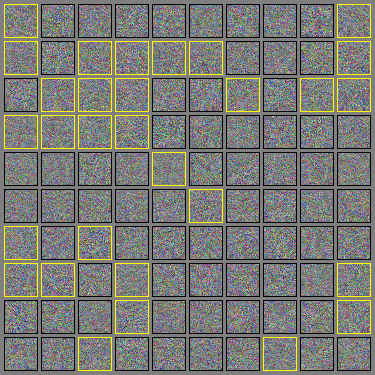
\includegraphics[height=2.5cm]{rubbish} 
\end{tabular}
\end{table}
\begin{itemize}
\pause
% \item Overconfidence alone does not fully explain why confidence is high
% on these non-sensical inputs. \pause
\item Overconfidence does not cover non-sensical inputs. \pause
\item Reduced examples are rubbish examples. \pause
\item \textbf{How did input reduction lead to rubbish examples?}
\end{itemize}
\end{frame}

\begin{frame} 
\begin{table}
\small
\begin{tabular}{p{0.72\columnwidth}l}
\textbf{\squad{}}  \\
\multicolumn{2}{p{0.9\columnwidth}}{The Panthers used the San Jose State practice facility and
stayed at the San Jose Marriott. The Broncos practiced at
\mybox{coloranswer}{Stanford University} and stayed at the Santa Clara
Marriott.} \\\\
Question & Confidence \\\midrule
Where did the {Broncos} practice for the Super Bowl ? & (0.90, 0.89) \pause\\
Where did the \textcolor{white}{Broncos} practice for the Super Bowl ? & (0.92, 0.88) \\
\end{tabular}
\end{table}
\begin{itemize}
\pause
\item Confidence remains high after the crucial word is removed.
\pause
\item Decrease in confidence does not align with importance.
\pause
\item After the first reduction step, the input is already rubbish.
\end{itemize}
\end{frame}

\begin{frame}
\textbf{\squad{}} \\
QuickBooks sponsored a ``Small Business Big Game'' contest, in
which Death Wish Coffee had a 30-second commercial aired free of
charge courtesy of QuickBooks. \mybox{coloranswer}{Death Wish
Coffee} beat out nine other contenders from across the United
States for the free advertisement. \newline \newline
%  \mybox{color1}{\strut{What}} \mybox{color1}{\strut{company}} \mybox{color1}{\strut{won}} \mybox{color1}{\strut{free}} \mybox{color6}{\strut{advertisement}} \mybox{color1}{\strut{due}} \mybox{color1}{\strut{to}} \mybox{color1}{\strut{QuickBooks}} \mybox{color0}{\strut{\underline{contest}}} \mybox{color1}{\strut{?}}\\
 \mybox{color1}{\strut{What}} \mybox{color1}{\strut{company}} \mybox{color1}{\strut{won}} \mybox{color1}{\strut{free}} \mybox{color6}{\strut{advertisement}} \mybox{color1}{\strut{due}} \mybox{color1}{\strut{to}} \mybox{color0}{\strut{\underline{QuickBooks}}} \mybox{color1}{\strut{?}}\\
 \mybox{color2}{\strut{What}} \mybox{color0}{\strut{company}} \mybox{color1}{\strut{won}} \mybox{color1}{\strut{free}} \mybox{color0}{\strut{\underline{advertisement}}} \mybox{color1}{\strut{due}} \mybox{color1}{\strut{to}} \mybox{color5}{\strut{?}}\\
 \pause
 \mybox{color1}{\strut{What}} \mybox{color0}{\strut{\underline{company}}} \mybox{color1}{\strut{won}} \mybox{color1}{\strut{free}} \mybox{color1}{\strut{due}} \mybox{color1}{\strut{to}} \mybox{color5}{\strut{?}}\\
 \mybox{color1}{\strut{What}} \mybox{color4}{\strut{won}} \mybox{color0}{\strut{\underline{free}}} \mybox{color1}{\strut{due}} \mybox{color0}{\strut{to}} \mybox{color5}{\strut{?}}\\
 \mybox{color1}{\strut{What}} \mybox{color1}{\strut{won}} \mybox{color1}{\strut{due}} \mybox{color1}{\strut{to}} \mybox{color0}{\strut{\underline{?}}}\\
 \mybox{color1}{\strut{What}} \mybox{color4}{\strut{won}} \mybox{color1}{\strut{due}} \mybox{color0}{\strut{\underline{to}}}\\
 \pause
 \mybox{color4}{\strut{What}} \mybox{color2}{\strut{won}} \mybox{color1}{\strut{\underline{due}}}\\
 \mybox{color2}{\strut{What}} \mybox{color1}{\strut{\underline{won}}}\\
 \mybox{color2}{\strut{What}}\\

\small
\mybox{color1}{\strut{What}} \mybox{color1}{\strut{company}}
\mybox{color1}{\strut{won}} \mybox{color1}{\strut{free}}
\mybox{color6}{\strut{advertisement}} \mybox{color1}{\strut{due}}
\mybox{color1}{\strut{to}} \mybox{color1}{\strut{QuickBooks}}
\mybox{color0}{\strut{{contest}}} \mybox{color1}{\strut{?}}\\\pause

\mybox{color1}{\strut{What}} \mybox{color1}{\strut{company}}
\mybox{color1}{\strut{won}} \mybox{color1}{\strut{free}}
\mybox{color6}{\strut{advertisement}} \mybox{color1}{\strut{due}}
\mybox{color1}{\strut{to}} \mybox{color0}{\strut{{QuickBooks}}}
\mybox{color1}{\strut{?}}\\\pause

\mybox{color2}{\strut{What}} \mybox{color0}{\strut{company}}
\mybox{color1}{\strut{won}} \mybox{color1}{\strut{free}}
\mybox{color0}{\strut{{advertisement}}} \mybox{color1}{\strut{due}}
\mybox{color1}{\strut{to}} \mybox{color5}{\strut{?}}\\\pause

\mybox{color1}{\strut{What}} \mybox{color0}{\strut{{company}}}
\mybox{color1}{\strut{won}} \mybox{color1}{\strut{free}}
\mybox{color1}{\strut{due}} \mybox{color1}{\strut{to}}
\mybox{color5}{\strut{?}}\\

\mybox{color1}{\strut{What}} \mybox{color4}{\strut{won}}
\mybox{color0}{\strut{{free}}} \mybox{color1}{\strut{due}}
\mybox{color0}{\strut{to}} \mybox{color5}{\strut{?}}\\

% \mybox{color1}{\strut{What}} \mybox{color1}{\strut{won}}
% \mybox{color1}{\strut{due}} \mybox{color1}{\strut{to}}
% \mybox{color0}{\strut{{?}}}\\
% 
% \mybox{color1}{\strut{What}} \mybox{color4}{\strut{won}}
% \mybox{color1}{\strut{due}} \mybox{color0}{\strut{{to}}}\\
% 
% \mybox{color4}{\strut{What}} \mybox{color2}{\strut{won}}
% \mybox{color1}{\strut{{due}}}\\
% 
% \mybox{color2}{\strut{What}} \mybox{color1}{\strut{{won}}}\\
% \mybox{color2}{\strut{What}}\\
\pause
\begin{itemize}
\item Independent word importance implicitly assumes bag-of-words.
\item Higher-order correlations are ignored.
\end{itemize}
\end{frame}
